\documentclass{standalone}

\usepackage[english]{babel}
\usepackage[linesnumbered, ruled, vlined]{algorithm2e}

\usepackage{caption}

% to create listings

\usepackage{listings, lstautogobble}
\lstset{
  autogobble=true,
  frame=single,
}

\lstdefinelanguage{coq}[Objective]{Caml}{
  morekeywords={Structure, Definition, Inductive, list, return},
  sensitive=true
}

% to define font size

\usepackage{ulem}
\usepackage{moresize}
\usepackage{anyfontsize}

% to use tikz and its libraries

\usepackage{tikz-timing}
\usetikztiminglibrary[dual arrows]{clockarrows}

\usepackage{tikz}

\usetikzlibrary{backgrounds}
\usetikzlibrary{positioning, calc, arrows, shapes, automata, petri, patterns}

% to use tikzmark, to place and refer to marks outside the current figure

\tikzset{every picture/.style={remember picture}}

% styles for transitions

\tikzset{transition/.append style={fill=black!20, thick}}
\tikzset{transition/.append style={fill=black!20, thick}}

% styles for test and inhib arcs.

\tikzstyle{test}=[pre, *-]
\tikzstyle{inhib}=[pre, o-]

% to use colors

\usepackage{xcolor}

%%%%%%%%%%%%%%%%%%%%%%%%%%%%%%%%%%%%%%%%%%%%%%%%%%
%                  BEGIN DOCUMENT                %
%%%%%%%%%%%%%%%%%%%%%%%%%%%%%%%%%%%%%%%%%%%%%%%%%%

\begin{document}

\tikzset{timing/font=\fontsize{40}{41}\selectfont}
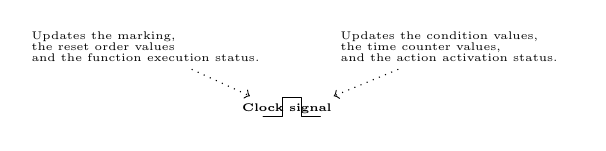
\begin{tikzpicture}
  \timing[name=clock] at (0, 0) {L2{C}};

  \node (clockcaption) at ([xshift=3mm, yshift=1mm]clock.origin) {
    \fontsize{4}{5}\selectfont \textbf{Clock signal}
  };
  
  % \node[circle, black, draw=black, inner sep=0.5mm] (fstep) at ([xshift=-15pt, yshift=7pt]clock.high mid) {
  %   \fontsize{4}{5}\selectfont 1
  % };

  \node[inner sep=0.5mm] (finstr) [above left= 5mm of clock.high mid] {
    \fontsize{4}{4}\selectfont
    \begin{tabular}{@{}l@{}}
      Updates the marking, \\
      the reset order values \\
      and the function execution status. \\
    \end{tabular}
  }
  edge[post, dotted] ($(clock.high mid)-(.5,0)$);
    
  \node[inner sep=0.5mm] (finstr) [above right= 5mm of clock.high mid] {
    \fontsize{4}{4}\selectfont
    \begin{tabular}{l}
      Updates the condition values, \\
      the time counter values, \\
      and the action activation status. \\
    \end{tabular}
  }
  edge[post, dotted] ($(clock.high mid)+(.5,0)$);  
\end{tikzpicture}

\end{document}
%%% Local Variables:
%%% mode: latex
%%% TeX-master: t
%%% End:
